\section{Compensated Horner scheme}

The "compensated" algorithms are an usual class of algorithm to increase the
program precision without changing the format. The rational is to capture at
every operation the accurate error term and to reinject it into the result.

In the Horner scheme, it is possible to retrieve at every step the error in
$x^2$ and the addition of the next coefficient by using respectively the
$Veltkamp-Dekker$ ({\tt twoProd}) for the product and $twoSum$ for the sum.
These algorithm are qualified as ({\it Error Free Transform}), EFT, in the
literature.

To better illustrate the concept, we can briefly analyze the $twoSum$ algorithm:
\begin{lstlisting}[frame=single, style=customC]
void twoSum (REAL a, REAL b,
              REAL &x, REAL &e) {
  x = a + b;
  const REAL z = x - a;
  e = (a - (x-z)) + (b-z);
}
\end{lstlisting}

The {\tt x} variable contain the FP sum of  {\tt a}  and  {\tt b} which can be written as $a+b+epsilon(a+b)$. \\
This epsilon is the error term corresponding to the absorption error on the result. \\
Therefore, we want to extract $ -epsilon(a+b)$ to capture the error term.  \\
The {\tt z} variable contains $b + epsilon(a+b)+epsilon(x-a)$. \\
Which makes {\tt a-(x-z)} contains $epsilon(x-a)+er^2$ and {\tt b-z} contains $-epsilon(a+b)-epsilon(x-a)+er^2$, $er^2$ is a term regrouping all error of the second order. \\
Finally {\tt e} will contain $-epsilon(a+b)$ with negligible second order terms.


{\tt twoProd} relies either on Dekker's algorithm, or on the IEEE FMA properties.
Dekker's algorithm will work on any architecture implementing IEEE floating point operators.
The listing is the following:
\begin{lstlisting}[frame=single, style=customC]
void Dekker (REAL x, Real y, Real &xy,  Real &er) {
  //extrapolated from http://toccata.lri.fr/gallery/Dekker.en.html
  #ifdef FLOAT
  REAL C=pow(2,12)+1
  #else
  REAL C==pow(2,27)+1
  #endif

  xy=x*y;

  //split x
  px=x*C;
  qx=x-px;
  hx=px+qx;
  tx=x-hx;

  //split y
  py=y*C;
  qy=y-py;
  hy=py+qy;
  ty=y-hy;

  //extract product error
  er=-xy+hx*hy;
  er+=hx*ty;
  er+=hy*tx;
  er+=tx*ty;
}
\end{lstlisting}

The algorithm for compensated horner scheme described in~\cite{graillat2005compensated} is the following:

\begin{algorithmic}[1]
  \Procedure{compHorner}{$x$,$\{a_1, a_2, \ldots, a_n\}$}
    \State {$s_n \gets a_n$}
    \State {$r_n \gets 0$}
    \For {$i \in [n-1:0]$}
       \State $[p_i, pe_i] \gets \text{\sc TwoProd}(s_{i+1}, x^2)$
       \State $[s_i, se_i] \gets \text{\sc TwoSum}(p_i, a_i)$
       \State $r_i \gets r_{i+1}\times x^2+(pe_i+se_i)$
    \EndFor
    \State \Return $s_0 + r_0$
  \EndProcedure
\end{algorithmic}

The lines 5 and 6, evaluates HORNER with EFT calls. Line 7 accumulate the error terms, which will be add to the final result on line 9.

\begin{question}
    \item Modify {\tt run.sh} to call comphorner with the following command: {\tt ./run.sh COMPHORNER FLOAT 24 }.
\end{question}

Instead of (carefully) recoding EFTs {\sc TwoProd} and {\sc TwoSum} manually, we suggest to use {\tt libeft}~\cite{libeft} available and documented at the following address: \url{https://github.com/ffevotte/libeft}.

\begin{question}
  \begin{enumerate}[(a)]
    \item Modify {\tt run.sh} to add libeft to the linker command. For this, just add {\tt -left} to verificarlo command and ensure that libeft path is in your  {\tt LIBRARY\_PATH}.
    \item Modify {\tt tchebychev.c} following that example:

      {
      \begin{lstlisting}[style=customC, basicstyle=\normalsize]
      #include <libeft.h>

      /* Define real type and format string */
      #ifdef DOUBLE
      #define REAL double
      #define FMT "%.16e %.16e"
      #define TWOPROD twoprod_d
      #define TWOSUM  twosum_d
      #else
      #define REAL float
      #define FMT "%.7e %.7e"
      #define TWOPROD twoprod_s
      #define TWOSUM  twosum_s
      #endif
      \end{lstlisting}
      }

     These modifications allow defining two macros corresponding to  {\tt TWOPROD} and {\tt TWOSUM} calling the EFT version according to the floating point format you are using.


    \item Implement {\tt REAL compHorner(REAL x)} in {\tt tchebychev.c} according to the comphorner algorithm provided in this tutorial. Modify the {\tt main} function to allow calling comphorner.
    \end{enumerate}
\end{question}


\begin{question}
  Evaluate {\tt compHorner} precision with Verificarlo. What happens if you use a precision different from 53 for program compiled in DOUBLE precision?

  $\Rightarrow$ WARNING, {\sc TwoProd} and {\sc TwoSum} relies on exact operations; it is essential to use RR 53 (Random Rounding with precision 53) mode of verificarlo for  \texttt{double} or RR 24 for \texttt{float}.
  \\~\\
  You should get the results of figures~\ref{fig:comphornerVerificarlo24} and \ref{fig:comphornerVerificarlo53}.
\end{question}

\begin{figure}[h!]
\center 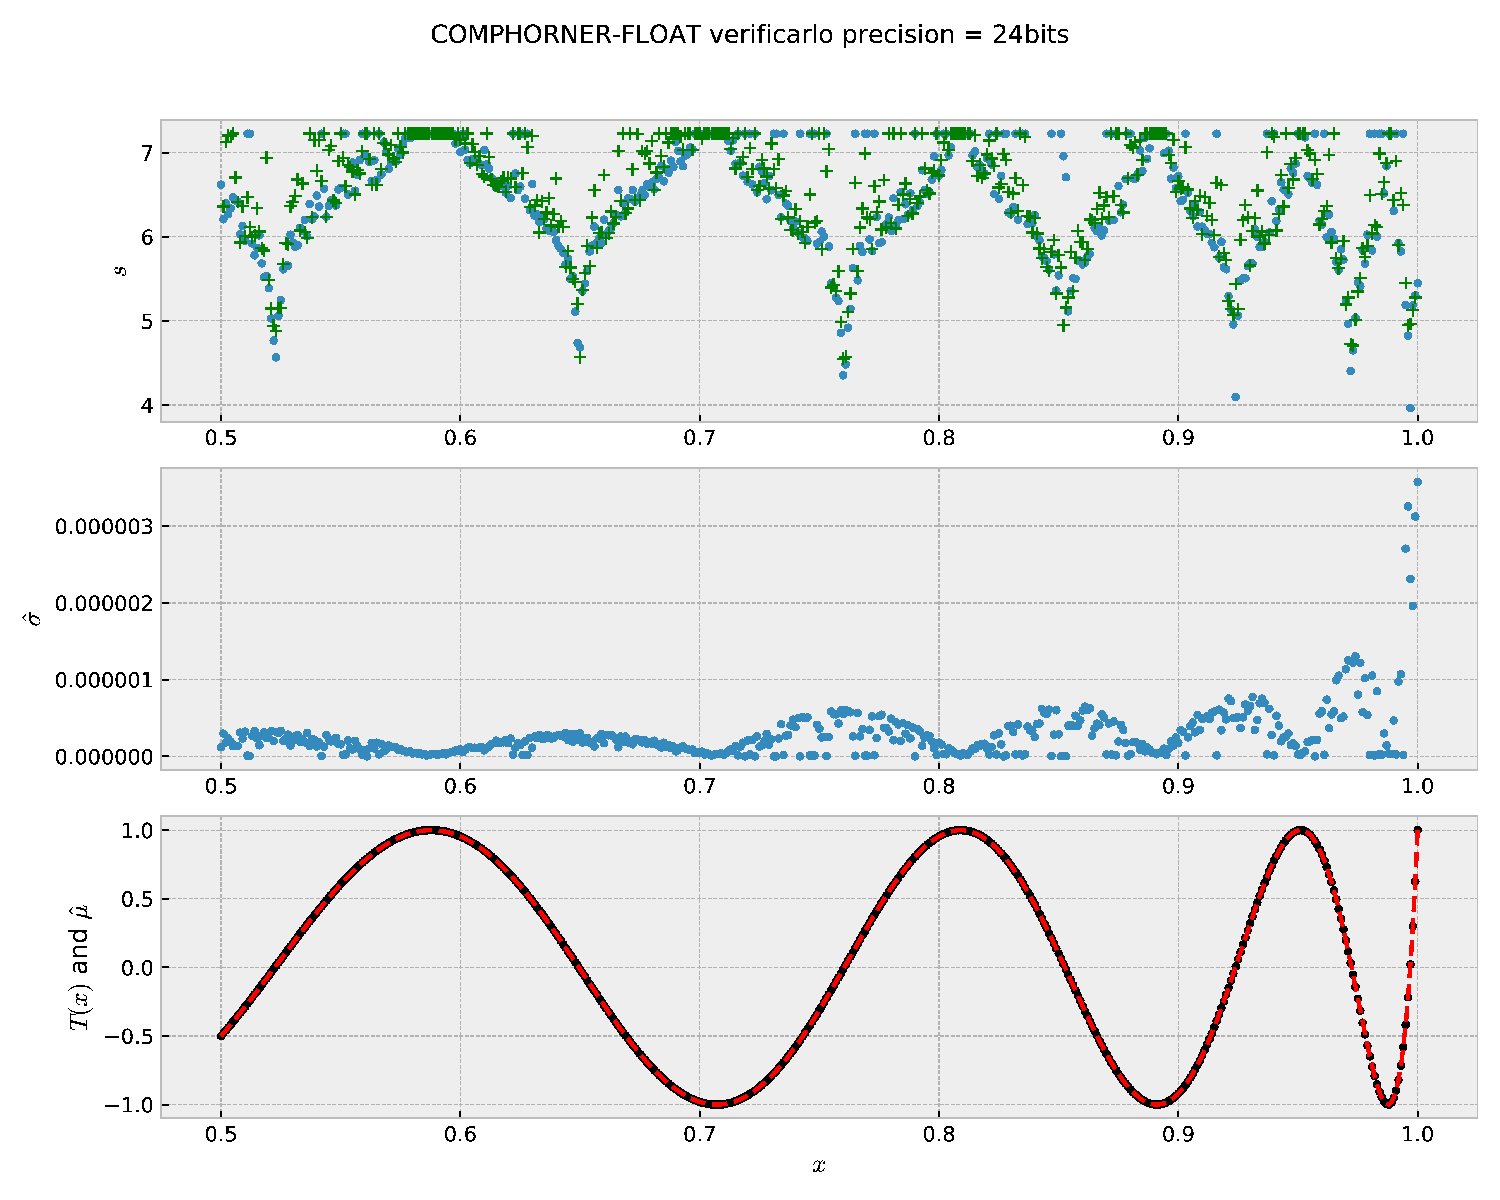
\includegraphics[width=.8\textwidth]{COMPHORNER-FLOAT-24+err.pdf}
  \caption{Evaluation of T(x) using Horner and compHorner in single precision: error estimated by verificarlo (blue), compared to the real error (green) }
  \label{fig:comphornerVerificarlo24}
\end{figure}

\begin{figure}[h!]
\center 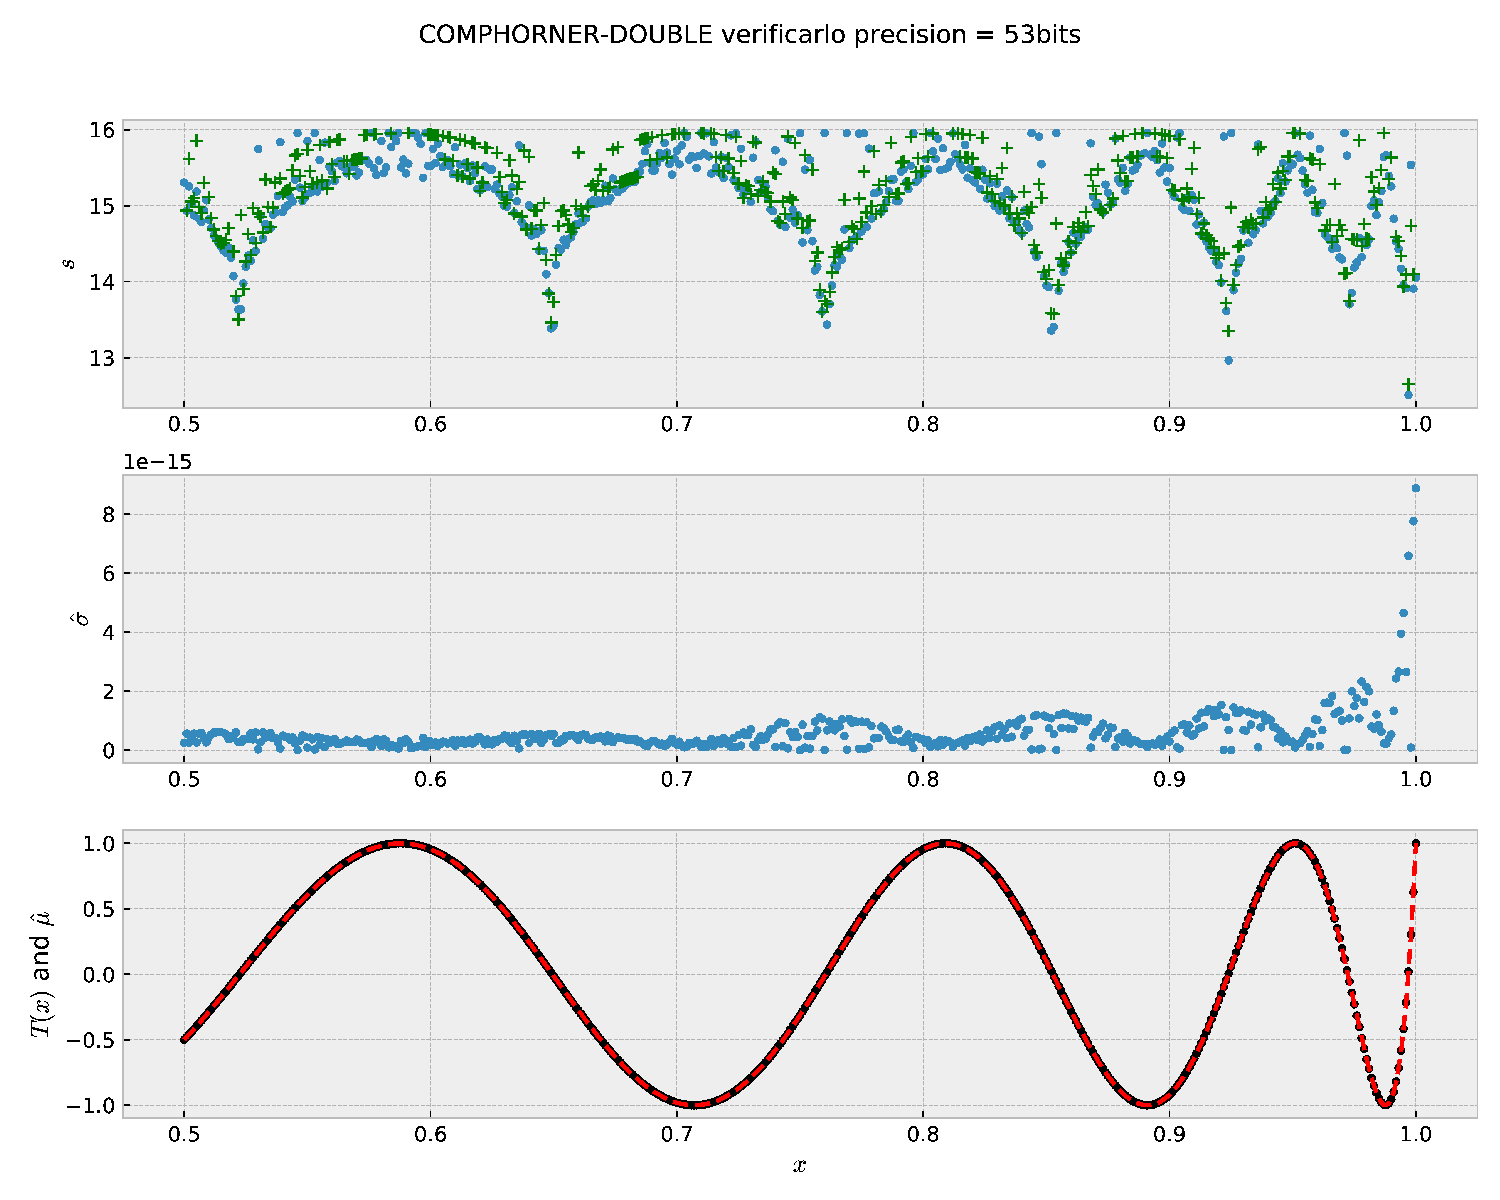
\includegraphics[width=.8\textwidth]{COMPHORNER-DOUBLE-53+err.pdf}
  \caption{Evaluation of T(x) using Horner and compHorner in double precision: error estimated by verificarlo (blue), compared to the real error (green)}
  \label{fig:comphornerVerificarlo53}
\end{figure}

The precision of this approach is given in figures~\ref{fig:comphornerVerificarlo24} and \ref{fig:comphornerVerificarlo53} with verificarlo.

We notice on the figures~\ref{fig:comphornerVerificarlo24} and \ref{fig:comphornerVerificarlo53} that CompHorner compensate precision losses in double and single precision. We retrieve a behavior similar to the factored form, in particularly for points $T(x)=1$. However, knowing the polynomial's roots for using the Horner scheme is not required.

In figures ~\ref{fig:comphornerVerificarlo24} and \ref{fig:comphornerVerificarlo53}, filled circles represent the real error value (evaluating in rational arithmetic in Python); circles represent the quality of the result computed in Monte Carlo Arithmetic with Verificarlo~\cite{verrou}.

First, at the cost of an increase number of operations, but, generally, in the same complexity class, it is possible to recover a part (or the full) precision lost. It exists algorithms called "accurate" that compute result without loss of precision, by, for example, recursively keeping errors terms until they can not be represented in the final result and that rounding is correct ({\it e.g.} $accSum$ of S. Hump).

Secondly, some algorithms, especially in mathematical libraries (libmath, Intel MKL, Intel VML, libeft) used particularity of the floating point format. By using Monte Carlo Arithmetic, it can be difficult even impossible to analyze them. In the random rounding specific case (as implemented by verificarlo RR mode with a precision length(mantissa)+1), a large amount of compensated algorithms can be analyzed (including compHorner as seen before). In addition, by their design, these algorithms have a proof of their level's precision correctness, which makes their evaluation by empirical methods useless.


